Spatial decompositions of a set of $d$ dimensional coordinates into a single
dimension is widely applied across computational science.
From forming the basis of implementations of finite-element methods, to algorithms
for mesh refinement, and importantly in our case, $N$-body simulations
\cite{Sundar:2008:SIAM}. Spatial decompositions utilise space-filling curves,
these infinite-curves are fractal, and by increasing their `order' can be made
to `fill', or describe, a $d$ dimensional space uniquely simply by their position
along the length of the curve \cite{Campbell:2003:Williams}. This concept is
illustrated in figure (\ref{fig:2_2_multi_order}) for the Morton encoding, or a
`Z-order' encoding.  This figure illustrates the fractal nature of a Morton
encoded line, with two `orders' of line encoding plotted over one another. We see
how by using a higher order encoding, we are able to to describe each position
in the domain of the box with a greater degree of precision, by using just
the length along the encoded line as a coordinate. This variant of space-filling
curves is used by \gls{PyExaFMM} as it better preserves the proximality of data
in the encoded coordinates than most other encodings, meaning that distance
between data points in physical space is preserved to an extent by the encoding. In $N$-Body
problems that use tree data structures, the encoded line is chosen to pass through
the centre of each box in the tree, at each level. Usefullly, Morton encodings
do not have the requirement to be continuous as illustrated by figure
(\ref{fig:2_2_multi_order}), making them relatively simple to implement.

As the line is chosen to pass through the center of each quadrant of the quadtree,
 the position along the line in each quadrant of a given box can be efficiently represented
 as a pair of `binary coordinates' corresponding to the index of the quadrant the line
 passes through, as the dimensions of the box at each level are pre-defined for a
 given octree. For example, the bottom-left quadrant at the coarser level in figure (\ref{fig:2_2_multi_order})
 will have a binary coordinate of,

 \begin{equation}
     \underbrace{0}_{x}\underbrace{0}_{y},
 \end{equation}

 where $x$ and $y$ correspond to the index of the quadrant along the $x$ and $y$
 directions at this level. This encoding can be made unique for each
 quadrant in each level by adding a displacement corresponding to the number of boxes so far
 encoded at all coarser levels. For example, the first encoded box, which in figure (\ref{fig:2_2_multi_order})
 corresponds to the binary coordinate $00$ will have a displacement of 0.
 This leaves this first box with a Morton encoded position, or \textbf{\gls{key}}
 of 0 in base ten. Similarly, the encoding for the bottom-left box at the finer
 level in figure (\ref{fig:2_2_multi_order}) will have binary coordinates of,

 \begin{equation}
    \underbrace{00}_{x}\underbrace{00}_{y},
\end{equation}

Four bits are needed, two each for the $x$ and $y$ coordinate, as there are 16
 quadrants at this level. The displacement due to the number of boxes encoded at
 previous levels of 4 \footnote{As is common in computer science, we begin indexing at 0, rather than 1.},
therefore it's Morton \gls{key} in base ten will be $4$. This concept is easily
extended to three dimensions, and is illustrated in
figure (\ref{fig:2_2_morton_encoding}) at level 1 of an octree. Here the binary
coordinates simply contain three bits, for the $xyz$ octant of a given cube
in the octree, and the displacement mechanism is entirely analogous with the
two dimensional case.

The binary coordinates of Morton encoded octants make it easy to perform simple
bitwise shift and comparison operations, to assign source and \gls{target-particles} to the Morton key
that encodes the octant they lie in for each level of a given octree, as well as traverse the levels of
the octree. Specifically, \gls{PyExaFMM} makes use of a \textit{linear} Morton encoding, meaning that it assigns
all particles to the keys of boxes they occupy at a maximum depth which has been refined to a
pre-defined leaf level of the desired octree. It does so by assuming that the
leaf level of the octree describing the domain of interest is partitioned into equal
sized leaf boxes, and checking the relative coordinates position of each particle
with respect to the expected indices of the leaf boxes. Furthermore, this operation only provides
a set of keys at the leaf-level which are non-empty, allowing \gls{PyExaFMM} to
ignore the remainder of the space covered by the domain of the octree. Once this
linear representation has been found, and the non-empty boxes containing
source and \gls{target-particles} identified, it's easy to traverse the octree
to find which ancestor boxes particles lie in by simply subtracting the appropriate
offset due to the box's position along the entire Morton encoded line, and adding a new offset at
at level of the ancestor box. The inverse operation can be done to provide the set
of keys corresponding to the descendent boxes for a given box. In terms of the
\gls{FMM} and \gls{KIFMM} algorithms, the above operations can be extended trivially
in simple combination to pre-compute \gls{interaction-list}s for each box, containing
only source boxes which aren't empty, as well as to find \gls{near-neighbours} of
a given box at a given level of the octree.

The power of encoding the domain of the octree lie in the optimisation opportunities
that arise. \gls{PyExaFMM} works entirely in terms of encoded Morton keys, using
them to lookup the correct precomputed operators, and store computational results against.
The ability to store an Morton encoding in Numpy vectors makes it possible to use
Numba's \textbf{\gls{JIT}} functionality to precompile the bitwise
operations, which are used heavily in \gls{PyExaFMM}'s implementation of the \gls{KIFMM}
main loop, mainly to traverse the octree. Properties of \gls{JIT} compilation are
elaborated on in Section \ref{sec:2_5_software_design}, and the speedup offered
by just-in-time compilation is benchmarked in Chapter \ref{chpt:3}, Section
\ref{sec:3_1_benchmarking}. Most significantly, this implementation detail
represents the first step towards optimising tree construction, with the
field of optimising highly-parallel tree constructions for octrees potentially containing
$10^9$ or more octree boxes, being an active area of research \cite{Sundar:2008:SIAM,Malhotra:2015:CCP}.
For example, the authors of PVFMM, one of the major C++ \gls{KIFMM} implementations,
evenly distribute the load of encoding particles for particularly deep octrees across
multiple processes using \gls{MPI} \cite{Malhotra:2015:CCP}. For highly non-uniform
data distributions the non-adaptive implementation of \gls{PyExaFMM} currently
will wastefully refine regions of the octree with a low density of particles, major
open source \gls{KIFMM} implementations thus implement adaptive tree refinement,
with different sized leaf boxes in different regions of the domain decsribed by
the octree \cite{Ying:2004:JCP, Malhotra:2015:CCP, exafmm}.

\begin{figure}[!h]
    \centering
    {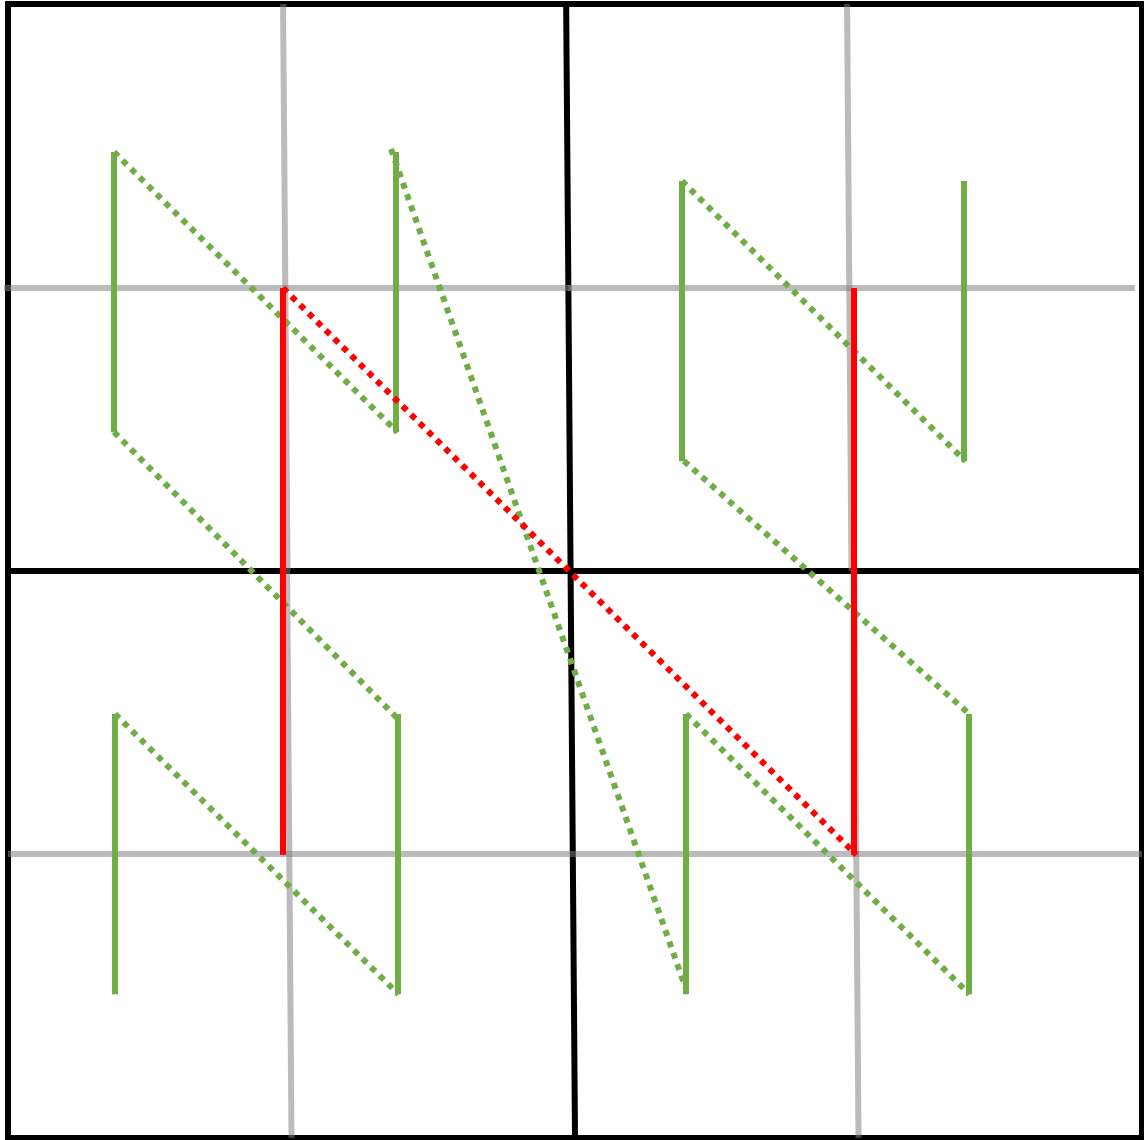
\includegraphics[width=0.45\textwidth]{chapter2/2_order.png}}
    \vspace{0pt}
    \caption{
        Two orders of Morton encoded lines in two dimensions for a quadtree across
        two adjacent levels. The red line encodes the center of the quadrants at the higher level,
        and and the green line encodes the corresponding points a level deeper.
        The dashed line indicates the order in which displacements are calculated
        in the encoding where the line is discontinuous.
    }
    \label{fig:2_2_multi_order}
\end{figure}


\begin{figure}[!h]
    \centering
    {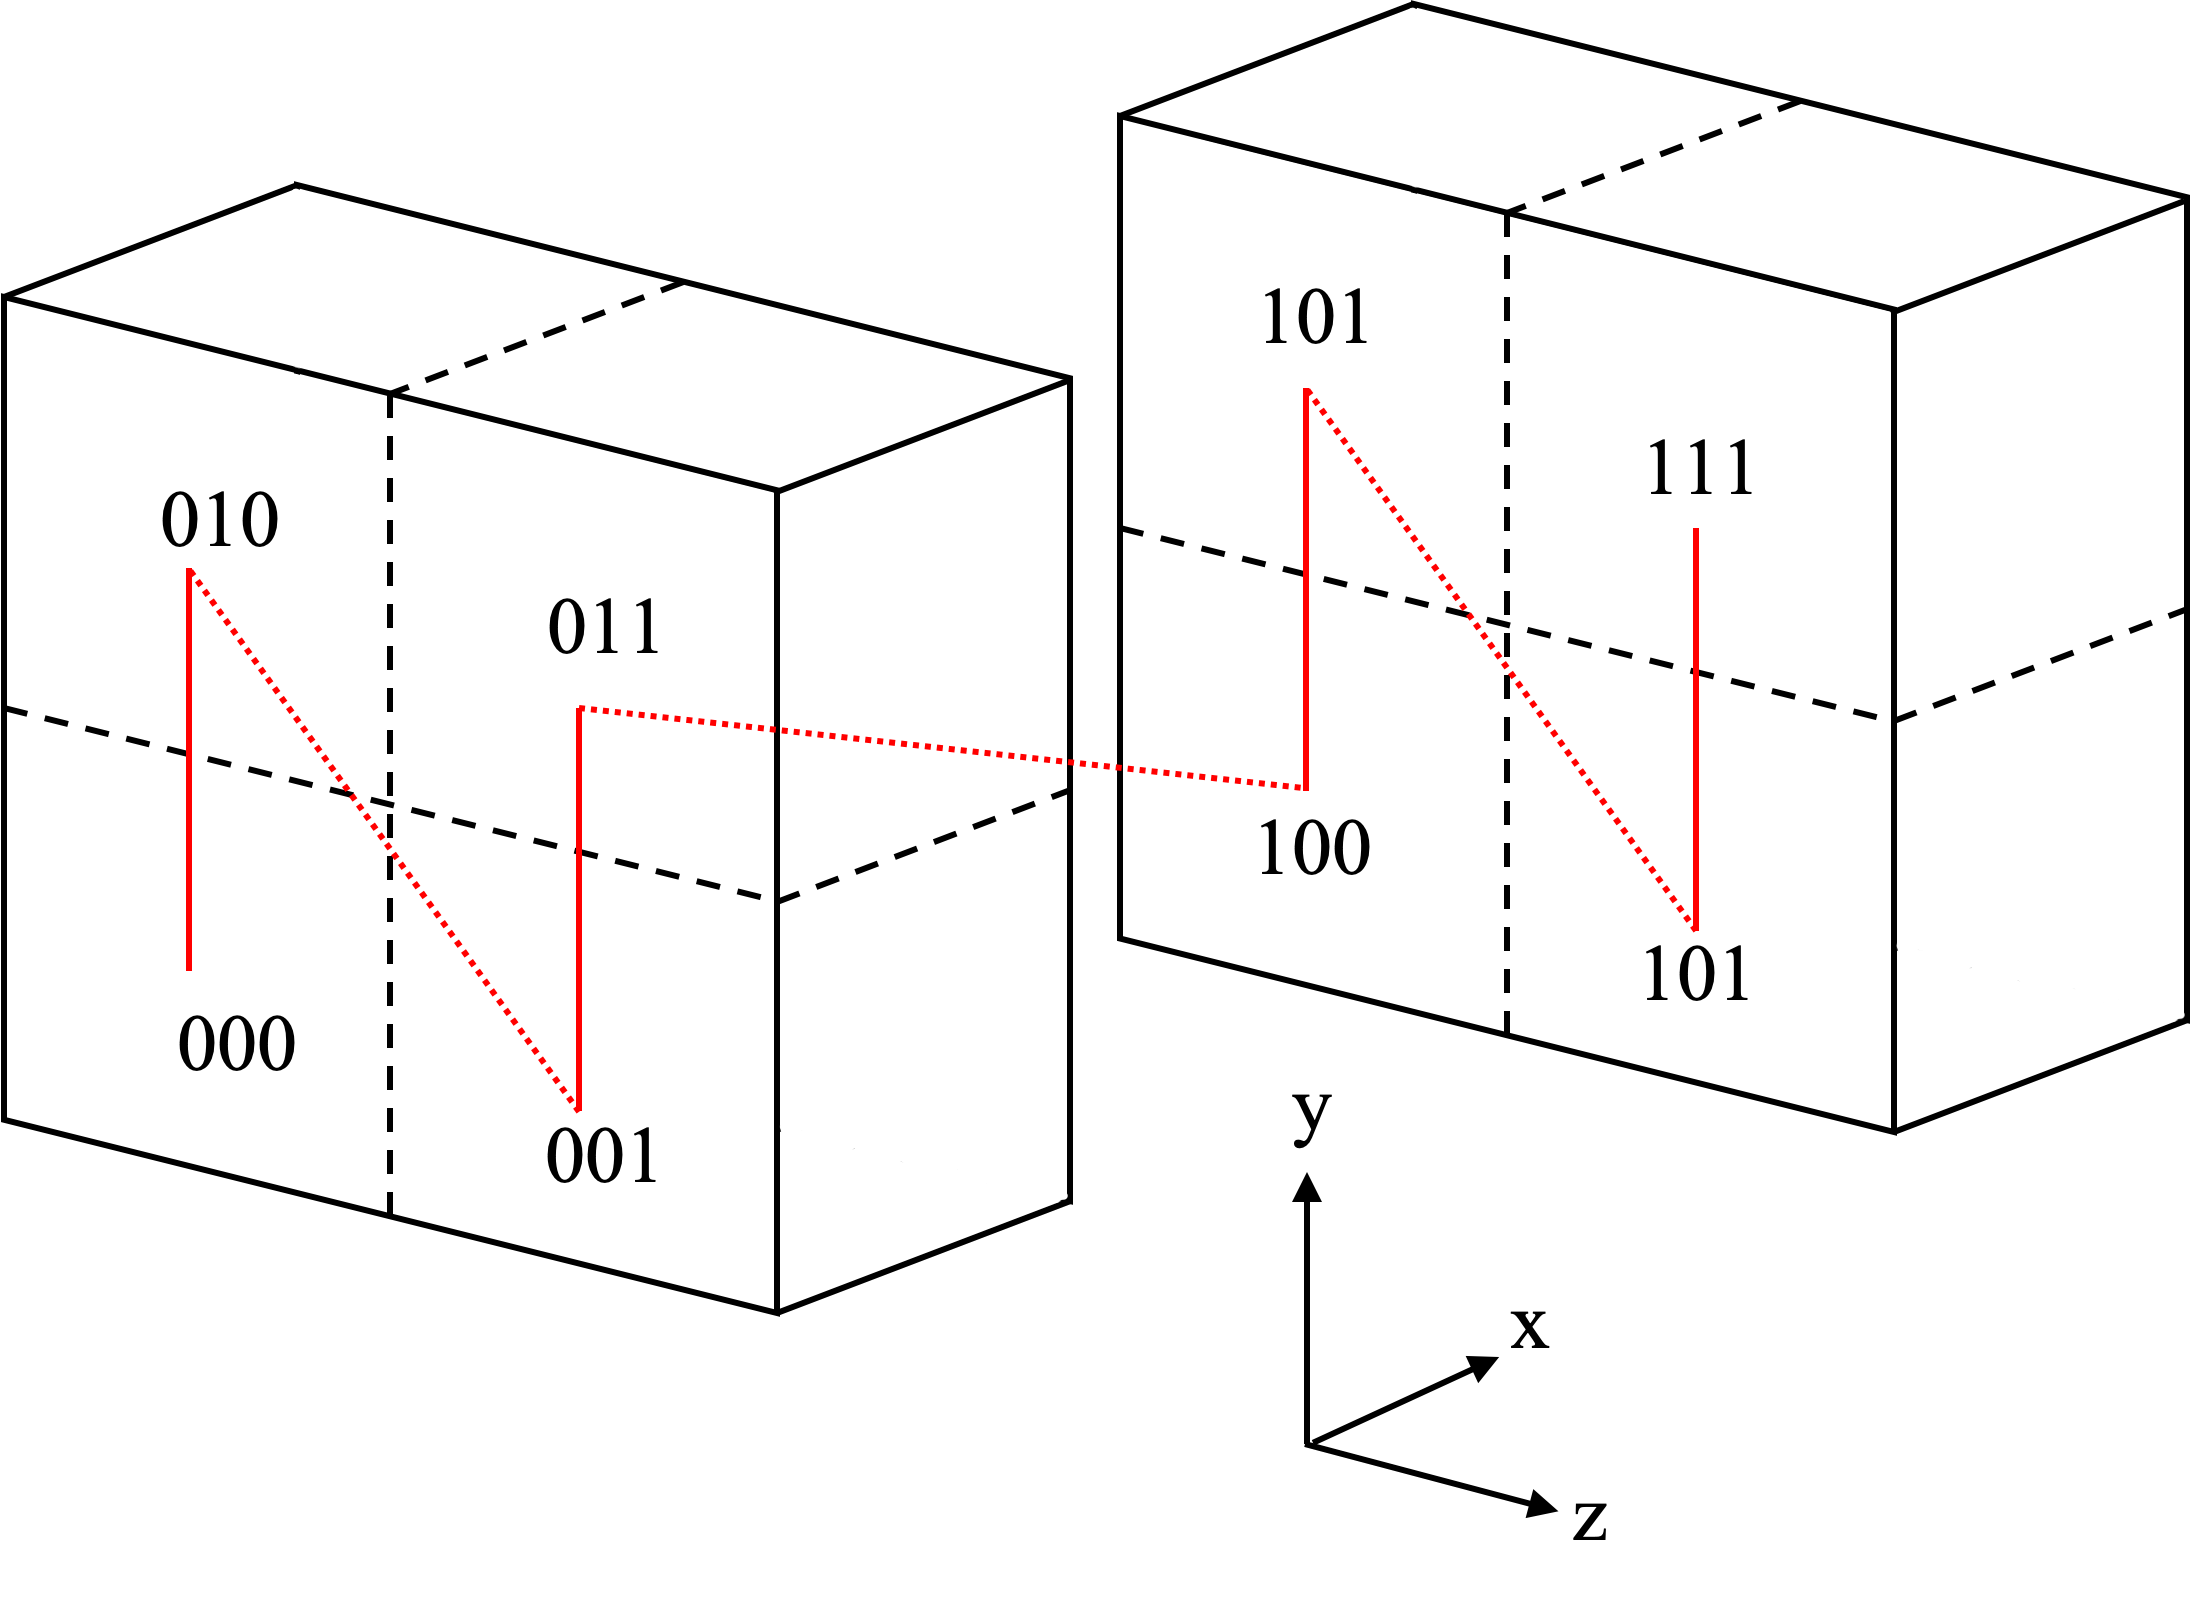
\includegraphics[width=0.65\textwidth]{chapter2/z_encoding.png}}
    \vspace{0pt}
    \caption{
        Morton encoding at level 1 of domain described by an non-adaptive octree.
        The two `layers' of the octree at this level have been broken apart
        in order to illustrate the encoded line. The Morton keys are written
        as binary coordinates in each octant.
    }
    \label{fig:2_2_morton_encoding}
\end{figure}